\documentclass[]{revdetua}
\usepackage{graphicx}
\usepackage{float}
\usepackage{listings}
\usepackage{xurl}

\begin{document}

\Header{Volume}{3}{Janeiro}{2022}{0}

\title{Advanced Algorithms Third Project \linebreak Most Frequent Letters}
\author{Daniela Dias 98039}
\maketitle

\begin{abstract}
This report studies different methods to identify the most frequent letters in text files. This problem is addressed by the course "Advanced Algorithms" at the University of Aveiro. The proposed approaches include Exact Counters, Approximate Counters, and the Misra-Gries algorithm (i.e. Frequent-Count, an algorithm to identify frequent items in data streams). Along with their implementation, we evaluate the quality of estimates regarding the exact counts and analyze the computational efficiency and limitations of the developed approaches. The chosen coding language was Python(3.11).
\end{abstract}

\begin{resumo}
Este relatório estuda diferentes métodos para identificar as letras mais frequentes em ficheiros de texto. Este problema é abordado pelo curso "Algoritmos Avançados" na Universidade de Aveiro. As abordagens propostas incluem Contadores Exatos, Contadores Aproximados e o algoritmo Misra-Gries (i.e. Frequent-Count, um algoritmo para identificar itens frequentes dentro de fluxos de dados). Juntamente com a sua implementação, nós avaliamos a qualidade das estimativas em relação às contagens exatas e analisamos a eficiência computacional e as limitações das abordagens. A linguagem de programação escolhida foi o Python(3.11).

\end{resumo}

\begin{keywords}% Note: in English (optional)
Letras Mais Frequentes, Processamento de Texto, Contador Exato, Contador Aproximado, Algoritmo  Misra-Gries, Frequent-Count
\end{keywords}

\begin{palavraschave}% Note: in Portuguese (optional)
Most Frequent Letters, Text Processing, Exact Counter, Approximate Counter, Misra-Gries Algorithm, Frequent-Count
\end{palavraschave}

\section{Introduction}

This report addresses the third project of "Advanced Algorithms", which requires us to identify the most frequent letters in text files using three different approaches: Exact counters, Approximate counters, and the Misra-Gries algorithm.

The first approach, exact counters, involves creating a frequency table (i.e. a dictionary) that counts the number of times each letter appears in the text file. This approach is straightforward and provides accurate results, serving as our reference point for comparing the results obtained by the Approximate Counters and the Misra and Gries algorithm.

The second approach, approximate counters, involves using a probabilistic data structure to estimate the frequencies of the most frequent letters. For this assignment, we implemented a decreasing probability counter (a variation of the mentioned approximate counters), which uses a probability of 1 / sqrt(2)\^k for each element in the stream. This approach allows for efficient memory usage, but the estimates may not be as accurate as the exact counts.

The third approach, the Misra and Gries algorithm, is a well-known algorithm for estimating the frequencies of the most frequent elements in data streams. It's an approach based on the idea of maintaining (k - 1) counters, one for each of the (k - 1) most frequent items, and processing the data stream one element at a time. It's another approach that allows for efficient memory usage, as it only requires (k - 1) counters, regardless of the data stream size. However, the estimates produced by the algorithm may not be as accurate as the exact frequencies, and the error tends to increase as the value of k decreases.

In this essay, we will analyze the computational efficiency and limitations of both Approximate Counters and the Misra-Gries algorithm, focusing on absolute and relative errors, average values, and the ability to identify the most frequent elements accurately. For this analysis, we must first compute the exact number of occurrences of all letters in the data stream (with the exact counters).

Afterward, we will estimate the frequency of the most frequent letters by running the Approximate counters a certain number of trials, with a probability of 1 / sqrt(2)\^k for each element in the stream. After running the algorithm 10 000 times, we will compare the results to the exact counts and calculate the absolute and relative errors. It will give us a sense of the overall accuracy of the algorithm and how well it performs compared to the exact counts. We will also verify whether the same most frequent letters are identified by the algorithm and in the same relative order. By performing a set of tests and repeating the approximate counts multiple times, we gain a deeper understanding of its strengths and weaknesses.

Next, we will estimate the (k - 1) most frequent letters by running the Misra and Gries algorithm for k = 3, k = 5, and k = 10. After running the algorithm, we will compare the results to the exact counts and calculate the accuracy for the (k-1) most frequent letters obtained. We can then evaluate the computational efficiency and limitations of the Misra and Gries algorithm by analyzing its accuracy.

Finally, we will test whether the most frequent letters identified by both algorithms are similar in the text files of the same literary work but in different languages. This study will give us insight into the generalization of the algorithms and whether they perform well in a variety of languages.

To generate the counters (and the statistics concerning processing times), run the following commands:

\begin{verbatim}
$ python exact_counter.py 
$ python approximate_counter.py
$ python data_stream_counter.py
\end{verbatim}

To compare the counters generated by the previous commands, run the following command:

\begin{verbatim}
$ python compare_counters.py
\end{verbatim}

\section{Text Processing}

For this assignment, we're asked to choose text files from literary works in different languages (as data for the computational experiments). Project Gutenberg is a well-known resource for obtaining such text files, with a large collection of public ebooks. We have decided to work with the ebook Alice’s Adventures in Wonderland in three different languages: English, German and French.

After obtaining the text files, we must process them to prepare for analysis. The first step in this procedure is to remove the Project Gutenberg file headers, which are added to the beginning of each ebook to provide additional information about the book (e.g. authors, illustrators, and translators). These headers can be identified by specific keywords and can be easily removed. We also removed the footers, with information about the source and licensing of the text, and all illustrations.

The next step is removing all stopwords and punctuation marks from the text. Stop words are common words that do not contribute much meaning to the text, such as articles, conjunctions, and prepositions. Removing stopwords can help reduce the size of the text and improve the efficiency of our algorithms. Punctuation marks, such as periods, commas, and exclamation points, are also removed to simplify the text and make it easier to process.

Finally, we remove all numbers, filter by alphabet letters, and convert the text to uppercase to ensure that all letters are in a consistent case. All these steps allow us to focus on the content of the text and perform a more efficient and accurate analysis.

In summary, to process the text files, we went through the following steps:
\begin{itemize}
\item Remove the Project Gutenberg file headers and footers.
\item Remove illustrations (appear with the text "[Illustration]").
\item Remove all stop-words.
\item Remove all punctuation marks, including apostrophes.
\item Remove all numbers.
\item Remove all letters outside of the English alphabet.
\item Convert all letters to uppercase.
\end{itemize}

The stop-words were obtained from an external repository [1].

\begin{table}[!ht]
    \centering
    Text Length Before and After Processing
    \begin{tabular}{|l|l|l|l|}
    \hline
        Language & Initial Length & Final Length & Difference \\ \hline
        English & 164013 & 56189 & 107824 \\ \hline
        German & 179151 & 130641 & 48510 \\ \hline
        French & 177112 & 127737 & 49375 \\ \hline
    \end{tabular}
\end{table}

On average, the text length decreased by 68570 letters.	 

\section{Exact Counter}

Exact counters, also known as exact frequency counters, are designed to provide an accurate count of the frequency of items in a dataset. We typically use these data structures when it is necessary to have a precise count of the number of occurrences of each item. In our case, we need to compare and evaluate the quality of estimates obtained by the other approaches.

In the context of identifying letters in a text file, we can use exact counters to count the real frequency of each letter. It is relevant for multiple purposes, such as analyzing the distribution of letters in a language or identifying common patterns in written communication. To implement exact counters for this task, we create a counter for each letter of the alphabet and increment the corresponding counter whenever we encounter that letter in the text. At the end of this process, the counters contain the accurate count of all letters.

One advantage of using exact counters for this task is that they provide an accurate count of the frequency of each letter. This can be important if we need the exact counts for further analysis (in particular, to analyze the results of other approaches) or if we're interested in knowing the distribution of letters in the text.

However, it's worth noting that exact counters can be slower and require more memory to store the count of each item. It is a limitation that becomes more significant if the dataset is large or if the processing speed is a concern. In such cases, an approximate counter may be a more suitable choice.

Finally, this data structure is also relevant for analyzing the similarity between the most frequent letters in the same literary work in different languages.

\begin{figure}[H]
    \centering
    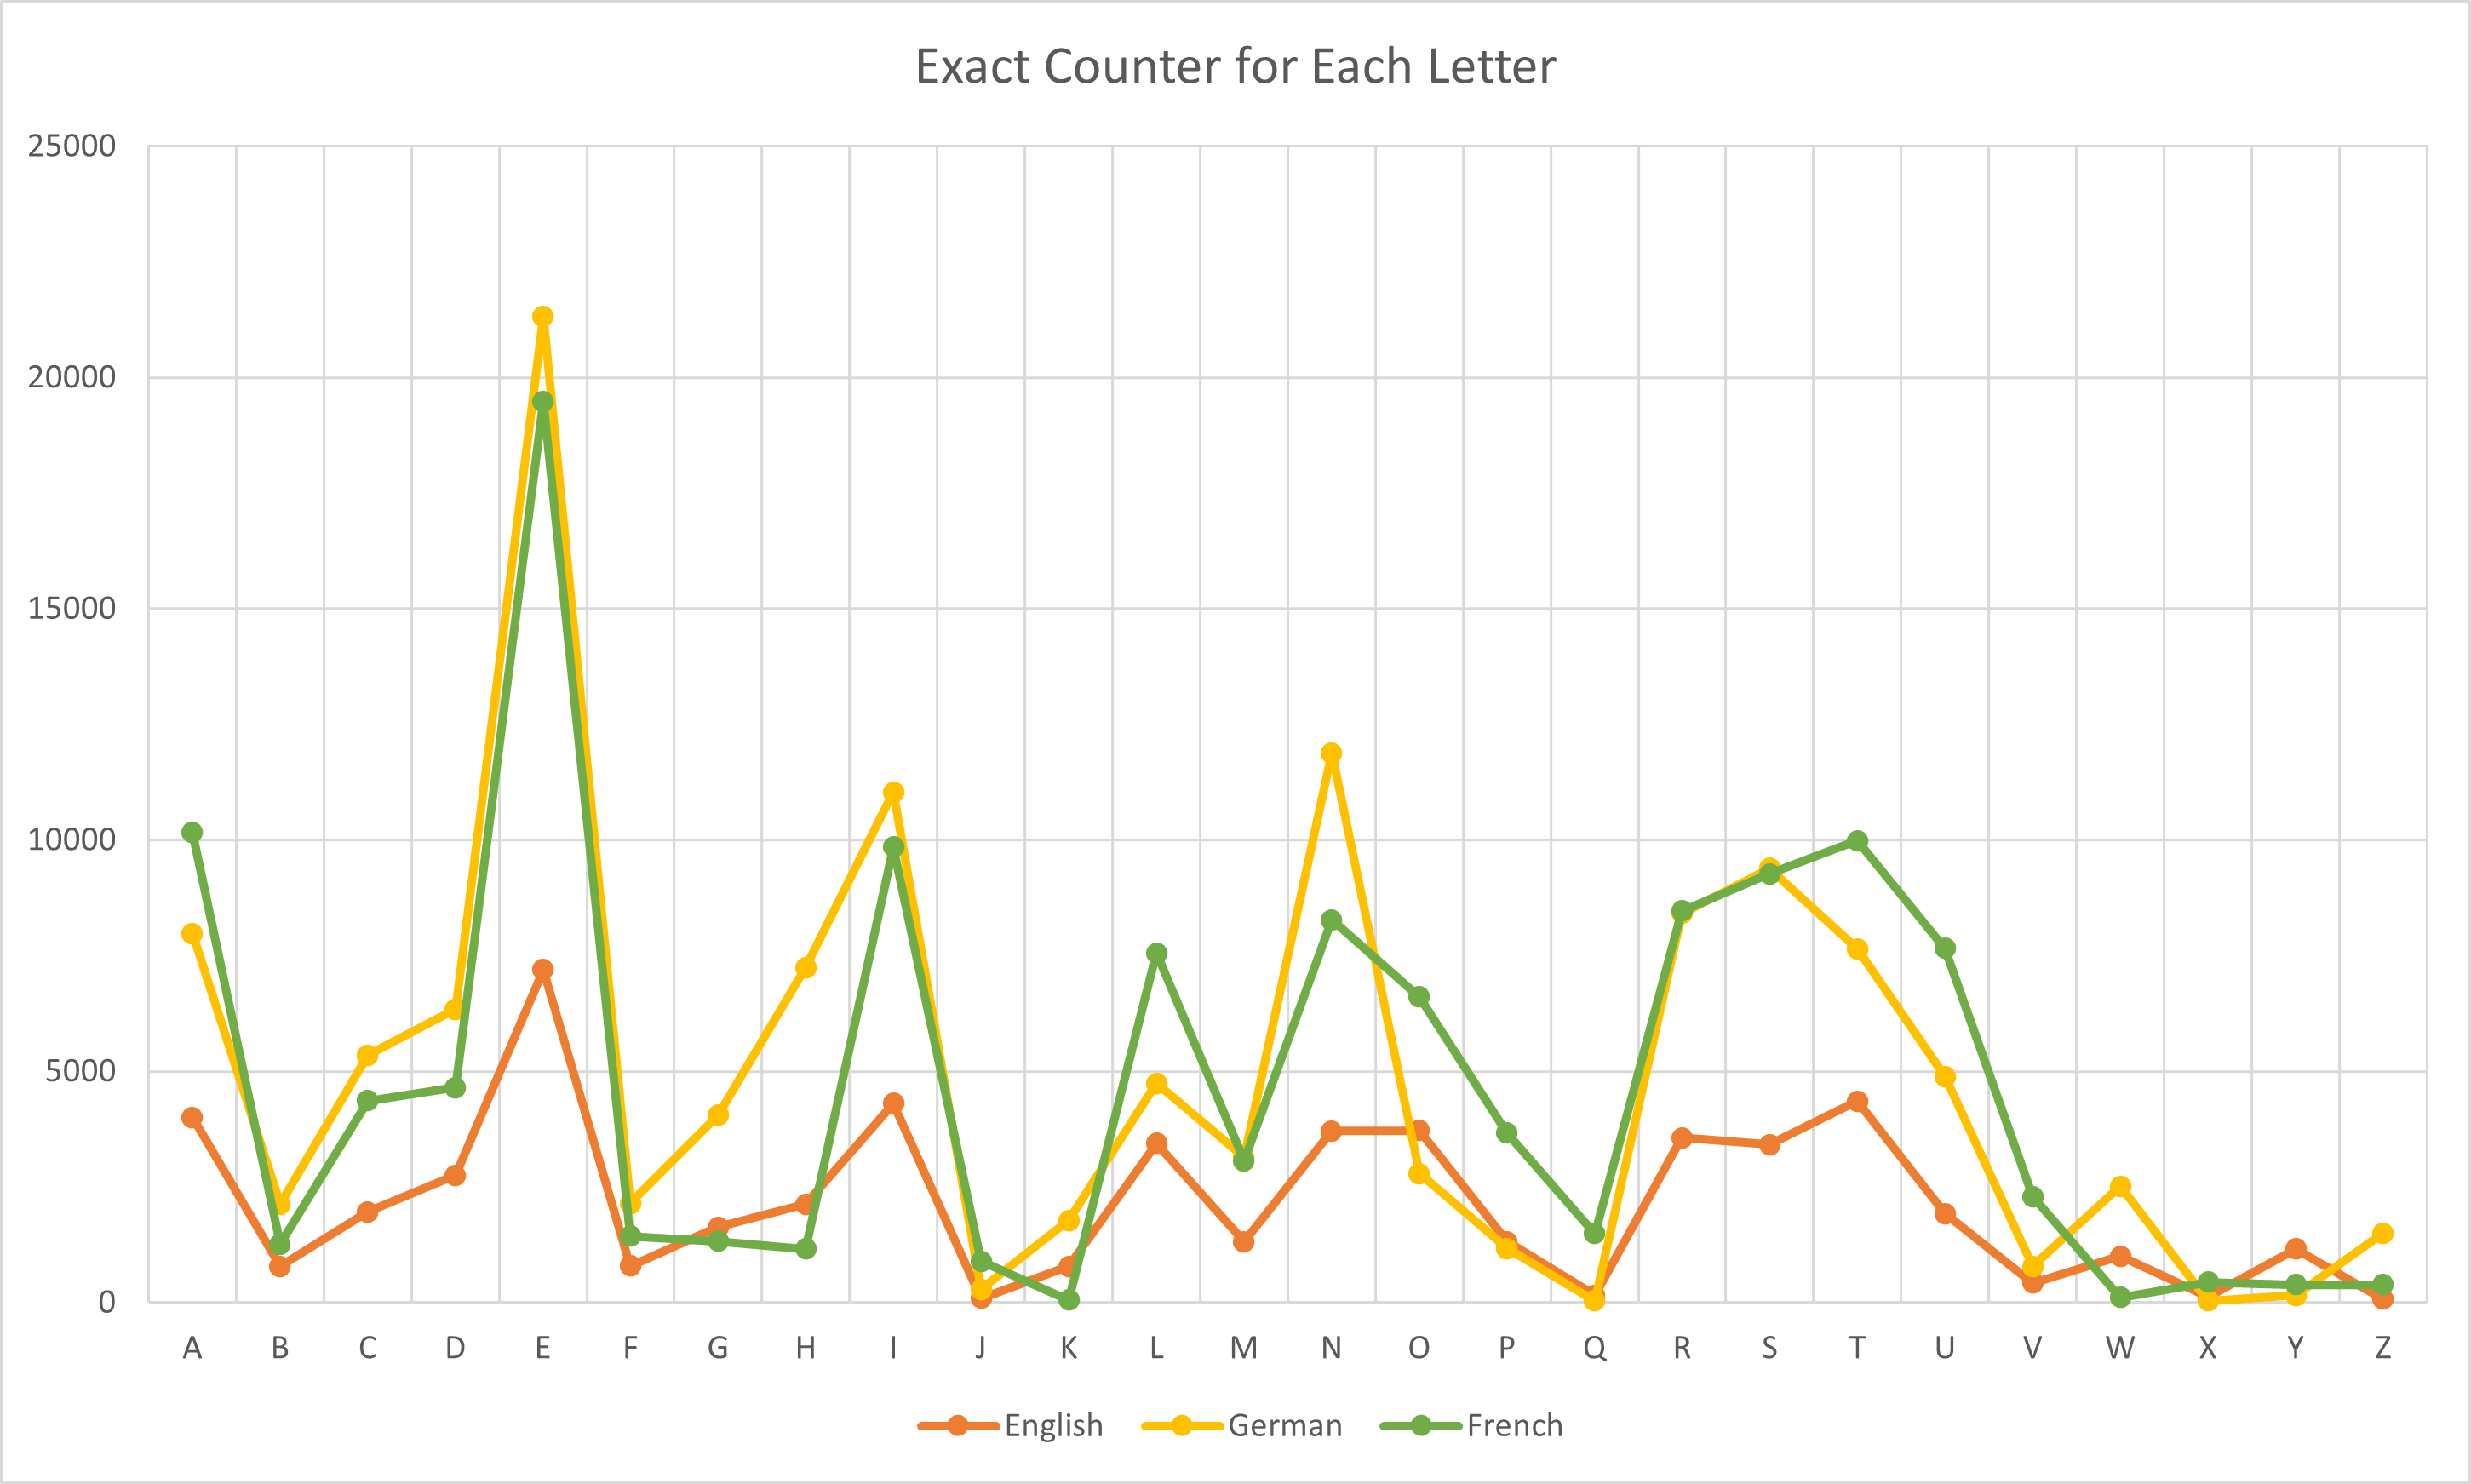
\includegraphics[width=8cm]{Exact Counter for Each Letter.png}
    \caption{Exact Counter for Each Letter}
\end{figure}

The letter "E" was the most frequent letter for the three languages (English, German and French), and the letters "T", "I" and "A" were in the six most frequent letters in common.

English Version:
{'E': 7201, 'T': 4360, 'I': 4314, 'A': 4005, 'O': 3720, 'N': 3715}

German Version:
{'E': 21330, 'N': 11884, 'I': 11040, 'S': 9393, 'R': 8412, 'A': 7978}

French Version
{'E': 19488, 'A': 10160, 'T': 9988, 'I': 9851, 'S': 9276, 'R': 8467}

\section{Approximate Counter}

Approximate counters are data structures designed to provide an approximate count of the frequency of items in a dataset. These counters trade off some accuracy for efficiency, as they can often process large amounts of data more quickly than exact counters. 

In the context of identifying letters in a text file, we can use approximate counters to estimate the frequency of each letter. This approach is practical for the same purposes as the exact counters (analyzing the distribution of letters or identifying common patterns in written communication). To implement an approximate counter for this task, we create a counter for each letter and increment the corresponding counter with a given probability whenever we encounter a letter. 

One advantage of using approximate counters is that they are faster and require less memory than exact counters. However, approximate counters are not as accurate as exact counters. They provide an estimate of the frequency of items rather than an exact count, which may not be suitable for all applications that require precise counts.

For this project, we implemented the approximate counters with decreasing probability: 1 / sqrt(2)\^k, where k is the count of the item (equivalent to the number of increments so far). One advantage of using decreasing probability is that it provides an approximate count of the frequency of items with a decreasing probability of error as the count increases. It is relevant when we need an approximate count with a high level of confidence in the accuracy of the most frequent letters. However, it is worth noting that it still is approximate.

We obtain the average results for a total number of 10 000 trials.

\begin{table}[!ht]
    \centering
    Absolute and Relative Errors For English Version\linebreak\linebreak
    \begin{tabular}{|l|l|}
    \hline
        ~ & English \\ \hline
        Expected value & 470.6177848 \\ \hline
        Variance & 235.3088924 \\ \hline
        Standard deviation & 15.33978137 \\ \hline
        Mean absolute error & 55723.4382 \\ \hline
        Mean relative error & 99.17143605 \\ \hline
        Mean accuracy ratio & 0.989256707 \\ \hline
        Smallest counter value & 435 \\ \hline
        Largest counter value & 489 \\ \hline
        Mean counter value & 465.5618 \\ \hline
        Mean absolute deviation & 4.95556852 \\ \hline
        Standard deviation & 6.212630744 \\ \hline
        Maximum deviation & 30.5618 \\ \hline
        Variance & 38.59678076 \\ \hline
    \end{tabular}
\end{table}

\begin{table}[!ht]
    \centering
    Absolute and Relative Errors For German Version\linebreak\linebreak
    \begin{tabular}{|l|l|}
    \hline
        ~ & German \\ \hline
        Expected value & 563.8654495 \\ \hline
        Variance & 281.9327248 \\ \hline
        Standard deviation & 16.79085241 \\ \hline
        Mean absolute error & 130082.7677 \\ \hline
        Mean relative error & 99.57269747 \% \\ \hline
        Mean accuracy ratio & 0.990009763 \% \\ \hline
        Smallest counter value & 537 \\ \hline
        Largest counter value & 581 \\ \hline
        Mean counter value & 558.2323 \\ \hline
        Mean absolute deviation & 5.1945336 \\ \hline
        Standard deviation & 6.493838365 \\ \hline
        Maximum deviation & 22.7677 \\ \hline
        Variance & 42.16993671 \\ \hline
    \end{tabular}
\end{table}

\begin{table}[!ht]
    \centering
    Absolute and Relative Errors For French Version\linebreak\linebreak
    \begin{tabular}{|l|l|}
    \hline
        ~ & French \\ \hline
        Expected value & 645.3023579 \\ \hline
        Variance & 322.651179 \\ \hline
        Standard deviation & 17.96249367 \\ \hline
        Mean absolute error & 127098.8035 \% \\ \hline
        Mean relative error & 99.50038243 \% \\ \hline
        Mean accuracy ratio & 0.988988328 \\ \hline
        Smallest counter value & 612 \\ \hline
        Largest counter value & 665 \\ \hline
        Mean counter value & 638.1965 \\ \hline
        Mean absolute deviation & 5.8322744 \\ \hline
        Standard deviation & 7.295059133 \\ \hline
        Maximum deviation & 26.8035 \\ \hline
        Variance & 53.21788775 \\ \hline
    \end{tabular}
\end{table}

\begin{table}[!ht]
    \centering
    Absolute and Relative Errors For Letter E (English)
    \begin{tabular}{|l|l|}
    \hline
        Letter & E (English) \\ \hline
        Expected value & 23.08525716 \\ \hline
        Variance & 11.54262858 \\ \hline
        Standard deviation & 3.397444419 \\ \hline
        Mean absolute error & 7178.1964 \\ \hline
        Mean relative error & 9968.332732 \% \\ \hline
        Mean accuracy ratio & 98.7799263 \% \\ \hline
        Smallest counter value & 19 \\ \hline
        Largest counter value & 28 \\ \hline
        Mean counter value & 22.8036 \\ \hline
        Mean absolute deviation & 0.96964464 \\ \hline
        Standard deviation & 1.220502782 \\ \hline
        Maximum deviation & 5.1964 \\ \hline
        Variance & 1.48962704 \\ \hline
    \end{tabular}
\end{table}

\begin{table}[!ht]
    \centering
    Absolute and Relative Errors For Letter E (German)
    \begin{tabular}{|l|l|}
    \hline
        Letter & E (German) \\ \hline
        Expected value & 26.21822135 \\ \hline
        Variance & 13.10911068 \\ \hline
        Standard deviation & 3.620650588 \\ \hline
        Mean absolute error & 21304.0445 \\ \hline
        Mean relative error & 9987.831458 \% \\ \hline
        Mean accuracy ratio & 98.9979436 \% \\ \hline
        Smallest counter value & 22 \\ \hline
        Largest counter value & 31 \\ \hline
        Mean counter value & 25.9555 \\ \hline
        Mean absolute deviation & 0.9286354 \\ \hline
        Standard deviation & 1.211412296 \\ \hline
        Maximum deviation & 5.0445 \\ \hline
        Variance & 1.46751975 \\ \hline
    \end{tabular}
\end{table}

\begin{table}[!ht]
    \centering
    Absolute and Relative Errors For Letter E (French)
    \begin{tabular}{|l|l|}
    \hline
        Letter & E (French) \\ \hline
        Expected value & 25.95763829 \\ \hline
        Variance & 12.97881914 \\ \hline
        Standard deviation & 3.602612822 \\ \hline
        Mean absolute error & 19462.3175 \\ \hline
        Mean relative error & 9986.821377 \% \\ \hline
        Mean accuracy ratio & 98.9400488 \\ \hline
        Smallest counter value & 21 \\ \hline
        Largest counter value & 30 \\ \hline
        Mean counter value & 25.6825 \\ \hline
        Mean absolute deviation & 0.98366 \\ \hline
        Standard deviation & 1.212226773 \\ \hline
        Maximum deviation & 4.6825 \\ \hline
        Variance & 1.46949375 \\ \hline
    \end{tabular}
\end{table}

\begin{table}[!ht]
    \centering
    Accuracy for Different Languages
    \begin{tabular}{|l|l|l|l|}
    \hline
        Language (Accuracy) & English & German & French \\ \hline
        Letter Order & 0.00\% & 0.00\% & 0.00\% \\ \hline
        Top 3 Char Order & 1.16\% & 2.57\% & 1.89\% \\ \hline
        Top 1 Char & 49.46\% & 79.15\% & 74.37\% \\ \hline
    \end{tabular}
\end{table}

\pagebreak

The tables show statistical values for the different language versions (English, German, French). These values include measures of central tendency (mean, expected value), dispersion (variance, standard deviation, mean absolute deviation), and accuracy (mean absolute error, mean relative error, mean accuracy ratio).

Overall, the results suggest that the approximate counters aren't as accurate as the exact counters for the three languages, as indicated by the high mean absolute error and mean relative error values. This approach performed poorly when identifying the most frequent orders of letters; however, it obtained the most frequent letter for all languages (letter "E") with relatively high accuracy.

\section{Misra-Gries Algorithm}

The Misra-Gries algorithm, also known as Frequent-Count, is a well-known method for finding the frequency of items in a data stream. It is a one-pass algorithm, meaning it only needs to process and run through the data stream once. At the same time, it is a simple and efficient algorithm with a wide range of applications, including natural language processing and database indexing.

One variation of the Misra-Gries algorithm is the Misra-Gries algorithm with the parameter k, which detects the (k-1) most frequent items in a data stream. We achieve this by maintaining (k - 1) counters (one for each of the k-1 most frequent items at a given time) and incrementing the corresponding counter whenever an item is processed. Here, the parameter k controls the quality of the results given. After all, we keep, at most, (k - 1) candidates at the same time, and we don't miss any item with (at least) frequency m / k. By allowing the detection of the (k - 1) most frequent items, the Misra-Gries algorithm with k provides more information about the distribution of elements in the stream.

One of the key advantages of the Misra-Gries algorithm is its efficiency. It can process large data streams in milliseconds, making it suitable for real-time applications. It is also relatively simple to implement, as it only requires a small number of counters and basic arithmetic operations. 

However, the Misra-Gries algorithm is not without its limitations. It is an approximate algorithm, meaning that it provides an estimate of the frequency of items rather than an exact count. This trade-off is necessary to achieve high efficiency, but it may not be suitable for all applications that require precise counts.

In our case, we apply this algorithm to estimate the (k - 1) most frequent letters in a processed text, for k = 3, k = 5, and k = 10.

\begin{table}[!ht]
    \centering
    Accuracy for the Misra-Gries algorithm
    \begin{tabular}{|l|l|l|l|}
    \hline
        Language & k & Correct Letters & Accuracy \\ \hline
        English & 3 & 0/2 & 0.00\% \\ \hline
        English & 5 & 2/4 & 50.00\% \\ \hline
        English & 10 & 4/9 & 44.44\% \\ \hline
        German & 3 & 0/2 & 0.00\% \\ \hline
        German & 5 & 1/4 & 25.00\% \\ \hline
        German & 10 & 4/9 & 44.44\% \\ \hline
        French & 3 & 0/2 & 0.00\% \\ \hline
        French & 5 & 1/4 & 25.00\% \\ \hline
        French & 10 & 4/9 & 44.44\% \\ \hline
    \end{tabular}
\end{table}

The accuracy is generally low, with an average accuracy of approximately 25-45\% across all languages and values of k. The accuracy is particularly low when k is small (k=3), with no correct letters identified in any language. As k increases, the accuracy improves slightly, but it remains relatively low overall. It is also worth noting that the accuracy is the same for all three languages when k is equal to 10. This could suggest that the Misra-Gries algorithm performs similarly for all languages at this value of k.

\section{Processing Time}

\begin{table}[!ht]
    \centering
    Exact Counters Time
    \begin{tabular}{|l|l|}
    \hline
        Title & Time \\ \hline
        Alice’s Adventures in Wonderland & 0.001963377 \\ \hline
        Alice's Abenteuer im Wunderland & 0.003954649 \\ \hline
        Aventures d'Alice au pays & 0.004023314 \\ \hline
    \end{tabular}
\end{table}

\begin{table}[!ht]
    \centering
    Approximate Counters (Average) Time
    \begin{tabular}{|l|l|}
    \hline
        Title & Time \\ \hline
        Alice’s Adventures in Wonderland & 0.201668063 \\ \hline
        Alice's Abenteuer im Wunderland & 0.42037122 \\ \hline
        Aventures d'Alice au pays & 0.877685649 \\ \hline
    \end{tabular}
\end{table}

\begin{table}[!ht]
    \centering
    The Misra-Gries Algorithm Time
    \begin{tabular}{|l|l|l|}
    \hline
        Title & k & Time \\ \hline
        Alice’s Adventures in Wonderland & 3 & 0.014958382 \\ \hline
        Alice’s Adventures in Wonderland & 5 & 0.013963699 \\ \hline
        Alice’s Adventures in Wonderland & 10 & 0.013991117 \\ \hline
        Alice's Abenteuer im Wunderland & 3 & 0.032430172 \\ \hline
        Alice's Abenteuer im Wunderland & 5 & 0.03291297 \\ \hline
        Alice's Abenteuer im Wunderland & 10 & 0.030918121 \\ \hline
        Aventures d'Alice au pays & 3 & 0.031464577 \\ \hline
        Aventures d'Alice au pays & 5 & 0.030886889 \\ \hline
        Aventures d'Alice au pays & 10 & 0.031915665 \\ \hline
    \end{tabular}
\end{table}

By analyzing the given tables, the Exact Counters and the Misra-Gries Algorithm had the best-performing times, always under 0.1 seconds.

\section{Conclusions}

In general, the choice between using an exact counter, an approximate counter, or the Misra-Gris algorithm depends on the specific requirements of the task at hand. If precise counts are necessary, exact counters are the better choice. However, if memory efficiency is more important, approximate counters or the Misra-Gries algorithm may be the better choice. 

Approximate counters are useful tools for estimating the frequency of items in a dataset, including the letters in a text. They require less memory; however, it was the slowest approach of the three due to the additional arithmetic operations to calculate the decreasing probability. With a fixed probability, the approximate counters would match the exact counters in speed.

Misra-Gries excels in speed and memory; however, it experimentally performed the worst. Despite its limitations, this algorithm remains a popular and widely used method for finding the frequency of items in a data stream. Its efficiency and simplicity make it a valuable tool for a wide range of applications.

\begin{thebibliography}{00}

\bibitem{b1} Lars Yencken. \textit{Stop-Words} [Online]. Available: \url{https://gist.github.com/larsyencken/1440509}
\bibitem{b2} James Schloss. \textit{The Approximate Counting Algorithm} [Online]. Available: \url{https://www.algorithm-archive.org/contents/approximate_counting/approximate_counting.html}
\bibitem{b3} Stéphane Guichard. \textit{The streaming model, and how to estimate the most frequent elements with the Misra-Gries algorithm.} [Online]. Available: \url{https://medium.com/nerd-for-tech/the-streaming-model-and-how-to-estimate-the-most-frequent-elements-with-the-misra-gries-algorithm-c880bbe7218b}

\end{thebibliography}

\end{document}
